\documentclass[12pt]{article}
\usepackage{tikz}
\usetikzlibrary{arrows.meta}
\usetikzlibrary{shapes.geometric}
\usetikzlibrary{shapes.symbols}
\usetikzlibrary{decorations,decorations.pathreplacing}
\usetikzlibrary{shadings}
\usetikzlibrary{backgrounds}
\usetikzlibrary{
  shapes,
  decorations.shapes,
  decorations.fractals,
  decorations.markings,
  shadows
}

\usepackage[utf8]{inputenc}
\usepackage{geometry}

\geometry{
  left=1cm,
  right=1cm,
  top=1.5cm,
  bottom=2.5cm
}

\usepackage{setspace}
\usepackage{xcolor}

\begin{document}

\begin{Large}
  \begin{singlespace}
    \begin{center}
      \textbf{Substrate Induction - Template} \\
      Version 1.0.0
    \end{center}
  \end{singlespace}
\end{Large}

\vspace*{10mm}

\begin{figure}[h]
  \begin{center}
    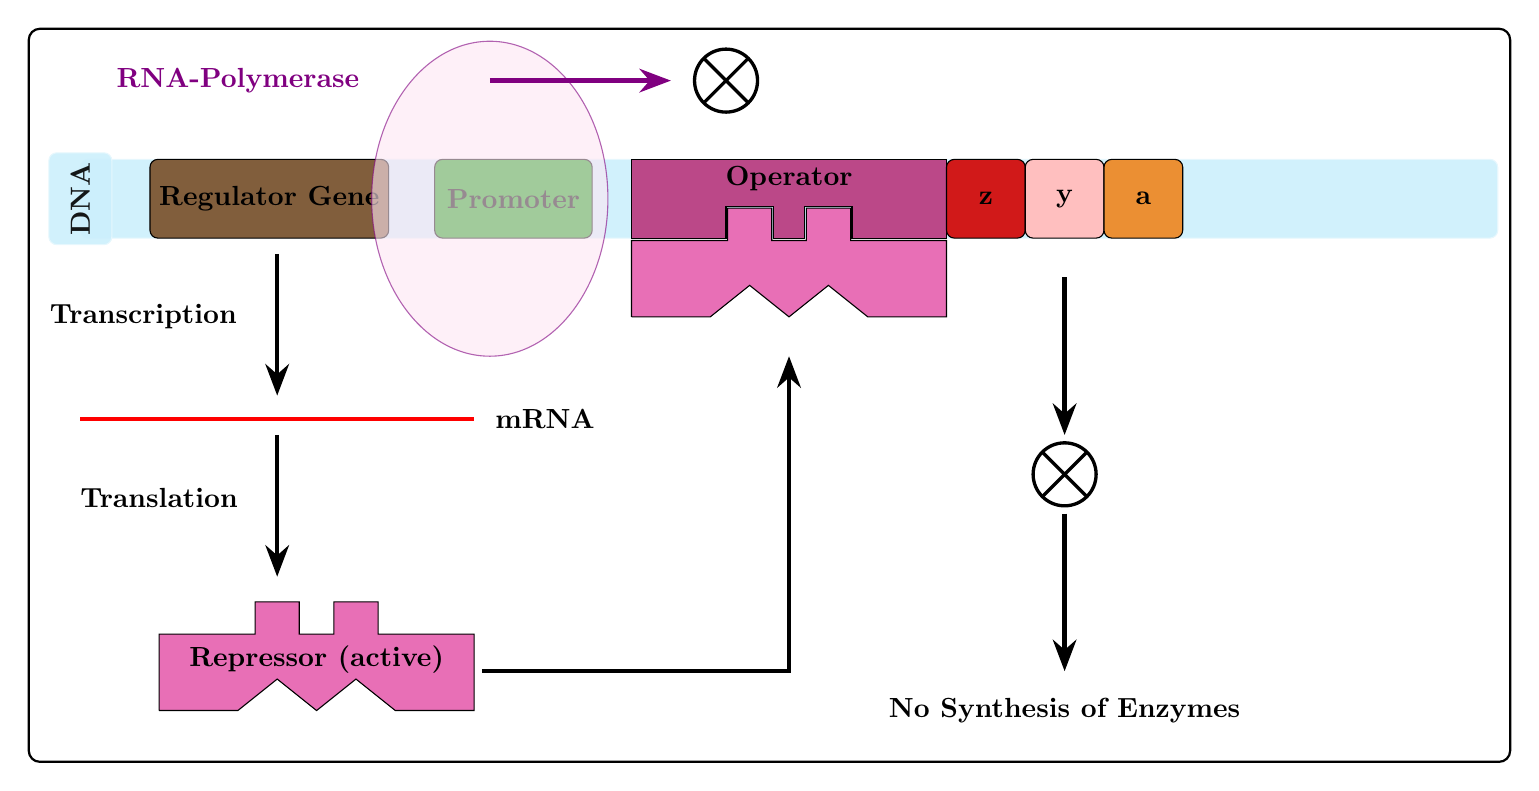
\begin{tikzpicture}[framed,background rectangle/.style={thick,draw=black, rounded corners},cross/.style={draw,path picture={
      \draw[black]
       (path picture bounding box.north west) -- (path picture bounding box.south east) 
       (path picture bounding box.south west) -- (path picture bounding box.north east);
      }}]
      %\draw[help lines] (-7,7) grid (7,-7); % Only for Development
    
      \node[shape=rectangle,
        rounded corners=1mm,
        draw=cyan!10,
        fill=cyan!20,
        fill opacity=0.9,
        minimum height = 1cm,
        minimum width = 18cm] at (0,0) {};
      \node[shape=rectangle,
        rounded corners=1mm,
        draw=cyan!10,
        fill=cyan!20,
        fill opacity=0.9,
        rotate=90,
        minimum height = 0.8cm,
        minimum width = 0.8cm] at (-9,0) {\textbf{DNA}};
      \node[shape=rectangle,
        rounded corners=1mm,
        draw=black,
        fill=brown!60!black!90,
        minimum height = 1cm,
        minimum width = 2cm] at (-6.6,0) {\textbf{Regulator Gene}};
      \node[shape=rectangle,
        rounded corners=1mm,
        draw=black,
        fill=green!60!black!90,
        minimum height = 1cm,
        minimum width = 2cm] at (-3.5,0) {\textbf{Promoter}};

      \node[shape=ellipse,
                        draw=violet,
                        rotate=90,
                        opacity=0.6,
                        fill=magenta!10,
                        minimum height = 3cm,
                        minimum width = 4cm] at (-3.8,0) {};
      \draw[-{Stealth[length=4mm]},ultra thick,draw=violet] (-3.8,1.5) -- (-1.5,1.5);
      \node [draw,circle,very thick,cross,minimum width=0.8cm] at (-0.8,1.5){}; 

      \node[shape=rectangle,
      text=violet,
      minimum height = 1cm,
      minimum width = 1cm] at (-7,1.5) {\textbf{RNA-Polymerase}};

      \draw[fill=magenta!70!black!90] 
        (-1,-0.5) -- (-2,-0.5) -- (-2,0.5) -- (2,0.5) -- 
        (2,-0.5) -- (0.8,-0.5) -- (0.8,-0.1) -- (0.2,-0.1) --
        (0.2,-0.5) -- (-0.2,-0.5) -- (-0.2,-0.1) -- (-0.8,-0.1) --
        (-0.8,-0.5) -- (-1,-0.5);

      \draw[fill=magenta!90!black!60]
        (-2,-1.5) -- (-2,-0.53) -- (-0.78,-0.53) -- (-0.78,-0.12) --
        (-0.22,-0.12) -- (-0.22,-0.53) -- (0.22,-0.53) -- (0.22,-0.12) --
        (0.782,-0.12) -- (0.782,-0.53) -- (2,-0.53) -- (2,-1.5) -- 
        (1,-1.5) -- (0.5,-1.1) -- (0,-1.5) -- (-0.5,-1.1) --
        (-1,-1.5) -- (-2,-1.5);

      \node[shape=rectangle,
        minimum height = 0.8cm,
        minimum width = 2cm] at (0,0.25) {\textbf{Operator}};

      \node[shape=rectangle,
        rounded corners=1mm,
        draw=black,
        fill=red!80!black!90,
        minimum height = 1cm,
        minimum width = 1cm] at (2.5,0) {\textbf{z}};
      \node[shape=rectangle,
        rounded corners=1mm,
        draw=black,
        fill=pink,
        minimum height = 1cm,
        minimum width = 1cm] at (3.5,0) {\textbf{y}};
      \node[shape=rectangle,
        rounded corners=1mm,
        draw=black,
        fill=orange!90!black!80,
        minimum height = 1cm,
        minimum width = 1cm] at (4.5,0) {\textbf{a}};

      \draw[-{Stealth[length=4mm]},ultra thick,draw=black] (3.5,-1) -- (3.5,-3);
      \node [draw,circle,very thick,cross,minimum width=0.8cm] at (3.5,-3.5){};
      \draw[-{Stealth[length=4mm]},ultra thick,draw=black] (3.5,-4) -- (3.5,-6);
      \node[shape=rectangle,
      minimum height = 1cm,
      minimum width = 1cm] at (3.5,-6.5) {\textbf{No Synthesis of Enzymes}};

      \draw[-{Stealth[length=4mm]},ultra thick,draw=black] (-6.5,-0.7) -- (-6.5,-2.5);
      \node[shape=rectangle,
        minimum height = 1cm,
        minimum width = 1cm] at (-8.2,-1.5) {\textbf{Transcription}};
        \draw[draw=red,ultra thick]
        (-9,-2.8) -- (-4,-2.8);
        \node[shape=rectangle,
        minimum height = 1cm,
        minimum width = 1cm] at (-3.1,-2.8) {\textbf{mRNA}};
      \draw[-{Stealth[length=4mm]},ultra thick,draw=black] (-6.5,-3) -- (-6.5,-4.8);
      \node[shape=rectangle,
        minimum height = 1cm,
        minimum width = 1cm] at (-8,-3.8) {\textbf{Translation}};
        
      \draw[fill=magenta!90!black!60]
        (-8,-6.5) -- (-8,-5.53) -- (-6.78,-5.53) -- (-6.78,-5.12) --
        (-6.22,-5.12) -- (-6.22,-5.53) -- (-5.78,-5.53) -- (-5.78,-5.12) --
        (-5.218,-5.12) -- (-5.218,-5.53) -- (-4,-5.53) -- (-4,-6.5) -- 
        (-5,-6.5) -- (-5.5,-6.1) -- (-6,-6.5) -- (-6.5,-6.1) --
        (-7,-6.5) -- (-8,-6.5);
      \node[shape=rectangle,
        minimum height = 1cm,
        minimum width = 1cm] at (-6,-5.85) {\textbf{Repressor (active)}};
      \draw[-{Stealth[length=4mm]},ultra thick,draw=black] (-3.9,-6) -- (0,-6) -- (0,-2);

    \end{tikzpicture}
  \end{center}
  \caption{Substrate Induction | blocked}
\end{figure}

\newpage

\begin{figure}[h]
  \begin{center}
    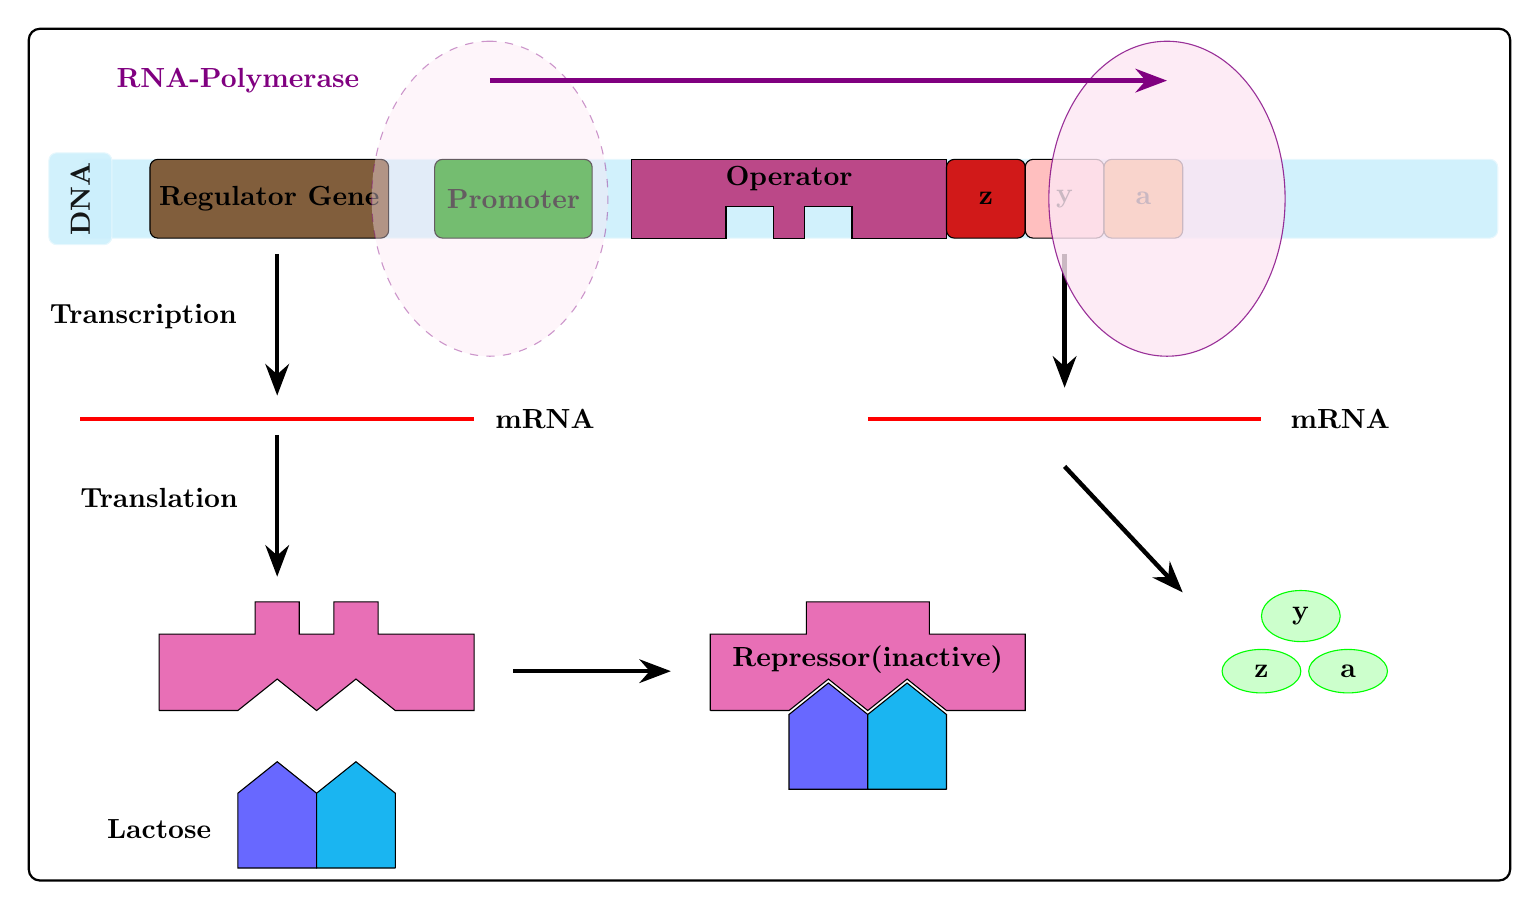
\begin{tikzpicture}[framed,background rectangle/.style={thick,draw=black, rounded corners},cross/.style={draw,path picture={
      \draw[black]
       (path picture bounding box.north west) -- (path picture bounding box.south east) 
       (path picture bounding box.south west) -- (path picture bounding box.north east);
      }}]
      %\draw[help lines] (-10,10) grid (10,-10); % Only for Development
    
      \node[shape=rectangle,
        rounded corners=1mm,
        draw=cyan!10,
        fill=cyan!20,
        fill opacity=0.9,
        minimum height = 1cm,
        minimum width = 18cm] at (0,0) {};
      \node[shape=rectangle,
        rounded corners=1mm,
        draw=cyan!10,
        fill=cyan!20,
        fill opacity=0.9,
        rotate=90,
        minimum height = 0.8cm,
        minimum width = 0.8cm] at (-9,0) {\textbf{DNA}};
      \node[shape=rectangle,
        rounded corners=1mm,
        draw=black,
        fill=brown!60!black!90,
        minimum height = 1cm,
        minimum width = 2cm] at (-6.6,0) {\textbf{Regulator Gene}};
      \node[shape=rectangle,
        rounded corners=1mm,
        draw=black,
        fill=green!60!black!90,
        minimum height = 1cm,
        minimum width = 2cm] at (-3.5,0) {\textbf{Promoter}};

      \node[shape=ellipse,dashed,
                        draw=violet,
                        rotate=90,
                        opacity=0.4,
                        fill=magenta!10,
                        minimum height = 3cm,
                        minimum width = 4cm] at (-3.8,0) {};
      
      \node[shape=rectangle,
      text=violet,
      minimum height = 1cm,
      minimum width = 1cm] at (-7,1.5) {\textbf{RNA-Polymerase}};

      \draw[fill=magenta!70!black!90] 
        (-1,-0.5) -- (-2,-0.5) -- (-2,0.5) -- (2,0.5) -- 
        (2,-0.5) -- (0.8,-0.5) -- (0.8,-0.1) -- (0.2,-0.1) --
        (0.2,-0.5) -- (-0.2,-0.5) -- (-0.2,-0.1) -- (-0.8,-0.1) --
        (-0.8,-0.5) -- (-1,-0.5);

      \node[shape=rectangle,
        minimum height = 0.8cm,
        minimum width = 2cm] at (0,0.25) {\textbf{Operator}};

      \node[shape=rectangle,
        rounded corners=1mm,
        draw=black,
        fill=red!80!black!90,
        minimum height = 1cm,
        minimum width = 1cm] at (2.5,0) {\textbf{z}};
      \node[shape=rectangle,
        rounded corners=1mm,
        draw=black,
        fill=pink,
        minimum height = 1cm,
        minimum width = 1cm] at (3.5,0) {\textbf{y}};
      \node[shape=rectangle,
        rounded corners=1mm,
        draw=black,
        fill=orange!90!black!80,
        minimum height = 1cm,
        minimum width = 1cm] at (4.5,0) {\textbf{a}};

      \draw[-{Stealth[length=4mm]},ultra thick,draw=black] (3.5,-0.7) -- (3.5,-2.4);
      \draw[-{Stealth[length=4mm]},ultra thick,draw=black] (3.5,-3.4) -- (5,-5);

      \node[shape=ellipse,
        draw=green,
        opacity=1,
        fill=green!20,
        minimum height = 0.5cm,
        minimum width = 1cm] at (6,-6) {\textbf{z}};
      \node[shape=ellipse,
        draw=green,
        opacity=1,
        fill=green!20,
        minimum height = 0.5cm,
        minimum width = 1cm] at (6.5,-5.3) {\textbf{y}};
      \node[shape=ellipse,
        draw=green,
        opacity=1,
        fill=green!20,
        minimum height = 0.5cm,
        minimum width = 1cm] at (7.1,-6) {\textbf{a}};

      \node[shape=ellipse,
        draw=violet,
        rotate=90,
        opacity=0.8,
        fill=magenta!10,
        minimum height = 3cm,
        minimum width = 4cm] at (4.8,0) {};
      \draw[-{Stealth[length=4mm]},ultra thick,draw=violet] (-3.8,1.5) -- (4.8,1.5);

      \draw[-{Stealth[length=4mm]},ultra thick,draw=black] (-6.5,-0.7) -- (-6.5,-2.5);
      \node[shape=rectangle,
        minimum height = 1cm,
        minimum width = 1cm] at (-8.2,-1.5) {\textbf{Transcription}};
      \draw[draw=red,ultra thick]
        (-9,-2.8) -- (-4,-2.8);
      \node[shape=rectangle,
        minimum height = 1cm,
        minimum width = 1cm] at (-3.1,-2.8) {\textbf{mRNA}};
      \draw[-{Stealth[length=4mm]},ultra thick,draw=black] (-6.5,-3) -- (-6.5,-4.8);
      \node[shape=rectangle,
        minimum height = 1cm,
        minimum width = 1cm] at (-8,-3.8) {\textbf{Translation}};
        
      \draw[fill=magenta!90!black!60]
        (-8,-6.5) -- (-8,-5.53) -- (-6.78,-5.53) -- (-6.78,-5.12) --
        (-6.22,-5.12) -- (-6.22,-5.53) -- (-5.78,-5.53) -- (-5.78,-5.12) --
        (-5.218,-5.12) -- (-5.218,-5.53) -- (-4,-5.53) -- (-4,-6.5) -- 
        (-5,-6.5) -- (-5.5,-6.1) -- (-6,-6.5) -- (-6.5,-6.1) --
        (-7,-6.5) -- (-8,-6.5);
     
      \draw[fill=blue!99!white!60]
        (-6,-8.5) -- (-7,-8.5) -- (-7,-7.55) -- (-6.5,-7.15) -- (-6,-7.55) -- (-6,-8.5);

      \draw[fill=cyan!90!]
        (-5,-8.5) -- (-6,-8.5) -- (-6,-7.55) -- (-5.5,-7.15) -- (-5,-7.55) -- (-5,-8.5);

      \node[shape=rectangle,
        minimum height = 1cm,
        minimum width = 1cm] at (-8,-8) {\textbf{Lactose}};

      \draw[-{Stealth[length=4mm]},ultra thick,draw=black] (-3.5,-6) -- (-1.5,-6);
        
      \draw[fill=magenta!90!black!60]
        (-1,-6.5) -- (-1,-5.53) -- (0.22,-5.53) -- (0.22,-5.12) --
        (0.78,-5.12) -- (1.22,-5.12) -- (1.782,-5.12) -- (1.782,-5.53) --
        (3,-5.53) -- (3,-6.5) -- (2,-6.5) -- (1.5,-6.1) -- 
        (1,-6.5) -- (0.5,-6.1) -- (0,-6.5) -- (-1,-6.5);
        
      \draw[draw=red,ultra thick]
        (1,-2.8) -- (6,-2.8);
      \node[shape=rectangle,
        minimum height = 1cm,
        minimum width = 1cm] at (7,-2.8) {\textbf{mRNA}};
      \node[shape=rectangle,
        minimum height = 1cm,
        minimum width = 1cm] at (1,-5.85) {\textbf{Repressor(inactive)}};

      \draw[fill=blue!99!white!60]
        (1,-7.5) -- (0,-7.5) -- (0,-6.55) -- (0.5,-6.15) -- (1,-6.55) -- (1,-7.5);

      \draw[fill=cyan!90!]
        (2,-7.5) -- (1,-7.5) -- (1,-6.55) -- (1.5,-6.15) -- (2,-6.55) -- (2,-7.5);

    \end{tikzpicture}
  \end{center}
  \caption{Substrate Induction | induced}
\end{figure}

\end{document}